\documentclass[11pt]{article}
\usepackage[margin=1in]{geometry}
\usepackage{amsmath,amssymb,amsthm}
\usepackage{graphicx}
\usepackage{float}
\usepackage{tikz}
\usetikzlibrary{arrows}
\usetikzlibrary{positioning}
\usepackage{fancyhdr}
\usepackage{listings}
\usepackage{algorithm}
\usepackage{algpseudocode}
\usepackage{titlesec}
\usepackage{hyperref}
\usepackage{epigraph}
\usepackage{caption}
\usepackage[
  backend=biber,
  style=authoryear,
  natbib=true
]{biblatex}

% Textbook-style
\titleformat{\section}{\normalfont\Large\bfseries}{\thesection.}{1em}{}
\titleformat{\subsection}{\normalfont\large\bfseries}{\thesubsection}{1em}{}

% Header
\pagestyle{fancy}
\fancyhf{}
\fancyhead[L]{Graph Algorithms}
\fancyhead[R]{HITS Algorithm}
\fancyfoot[C]{\thepage}
\setlength{\headheight}{14pt}

% Quote
\renewcommand{\epigraphflush}{center}
\setlength\epigraphwidth{0.8\textwidth}
\setlength\epigraphrule{0pt}

% References
\addbibresource{references.bib}

\title{Hyperlink-Induced Topic Search (HITS)}
\author{Ainslee Archibald \\ Graph Algorithms Final Project}
\date{}

\begin{document}

\maketitle

\epigraph{%
\textit{Moreover, it can be viewed as an intricate form of populist hypermedia, in which millions of on-line participants, with diverse and often conflicting goals, are continuously creating hyperlinked content.}%
}{--- Jon \textcite{kleinberg_authoritative_1999}, on the nature of the World Wide Web}

\section{Introduction}
Hyperlink-Induced Topic Search (HITS) is a foundational link analysis algorithm used to rank documents based on their connections in a hub and authority model of a network.
The algorithm was developed by Jon Kleinberg during his time at IBM \parencite{kleinberg_method_2000}, first presented at the ACM-SIAM Symposium on Discrete Algorithms in 1998 \parencite{kleinberg_authoritative_1998}, and later published in the Journal of the ACM in 1999 \parencite{kleinberg_authoritative_1999}.

PageRank was developed concurrently and cites Kleinberg \parencite{brin_anatomy_1998}.
Although HITS shares several similarities with PageRank, it is significantly less well-known and less widely used.

% TODO: refactor into 2-3 sentence summary of how it works
The algorithm formalizes a notion of authority based on the relationship between authoritative pages that provide content relevant to a topic and the hub pages that aggregate them with links.
If the creator of page $p$ links to page $q$, they have conferred some measure of authority onto $q$.
However, it is also important to make sure that $q$ is relevant to the query at hand, so a pure measure of popularity (lots of $p$ links) is not sufficient to return useful results.
Given a network graph and a set of pages relevant to a search query, HITS uses the link structure to find small collections of pages likely to contain the most authoritative pages on the topic, then calculates scores which represent the quality of these pages as either "hubs" or "authorities."

Applications include citation analysis, where resource (authority) quality can be analyzed both by number of citations and the quality of the citing resources (hubs), and web search ranking, where it is better for a page (authority) to receive links from higher quality aggregators (hubs).

\section{Problem Statement}
A collection $V$ of pages can be represented as a directed graph \( G = (V, E) \), with $(p, q) \in E$ if there exists a link from $p$ to $q$. 
In this formulation, the out-degree of page $p$ is the number of pages it links to, and the in-degree of $p$ is the number of pages that link to it.
A subset of pages $W \subseteq V$ has graph $G[W]$ with all the pages in $W$ and all the edges between pages in $W$.

\subsection{Input}
The input of HITS is a set of pages.
Before running the algorithm, then, a set of pages should be built that is relatively small, is rich in relevant pages, and contains most (or many) of the strongest authorities, in order to lower computational costs.

To do this, first gather a root set $R_\sigma$ of the highest-ranked pages for a query $\sigma$ from an existing search engine.
In the foundational paper by \textcite{kleinberg_authoritative_1999}, the search engines mentioned are AltaVista and Hotbot, so we can assume with some confidence that while this initial set will be sufficiently small and have only relevant pages, it is unlikely to contain most of the strongest authorities, because it is the late 90s, and search engines are not very good.

To make sure to bring in those strongest authorities (so that HITS can later identify and rank them), iterate through all the pages $p$ in $R_\sigma$.
For each $p$, add all pages that $p$ links to ($\Gamma^+(p)$) and all pages that link to $p$ ($\Gamma^-(p)$).
In order to avoid growing $R_\sigma$ too large by adding every site that links to very popular sites, a restriction can be placed on how many pages in $\Gamma^-(p)$ can be added for any given $p$.
Call this newly constructed set the base set $S_\sigma$.

One more step should be taken to clean this base set of navigational links within websites, as these usually do not encode information useful to the hubs and authorities model.
This can be done by deleting any edges in $G[S_\sigma]$ between pages with the same domain name, resulting in the graph $G_\sigma$.
Additional steps can be taken to clean the graph and less useful information, but this is as far as Kleinberg went for the experiments in his original paper on HITS, so we shall move on to the outputs of the algorithm.

\subsection{Output}
The output of HITS can be thought about in a few ways, but the most general version simply assigns each page an authority weight $a_p$ and hub weight $h_p$.
These scores are non-negative and normalized so that each set sums to 1.
Pages with higher $a$- and $h$-values can be interpreted as being better authorities or hubs respectively.
Now, we shall discuss how to find these scores.

\section{Algorithm}
As mentioned previously, ranking purely by in-degree, even on our constructed $G_\sigma$, is likely to return many pages that are universally popular without being strong authorities for query $\sigma$.
However, we might expect that in addition to high in-degree, there would be overlap in the "hub" pages that link \textit{to} these authoritative pages.
A toy example of this relationship can be seen in Figure \ref{fig:hub-auth}.
In order to find the pages that are authoritative for $\sigma$, without using the textual content of the pages, HITS scores hubs that pull together many good authorities, and authorities that are linked to by many good hubs.

\begin{figure}[ht]
\centering
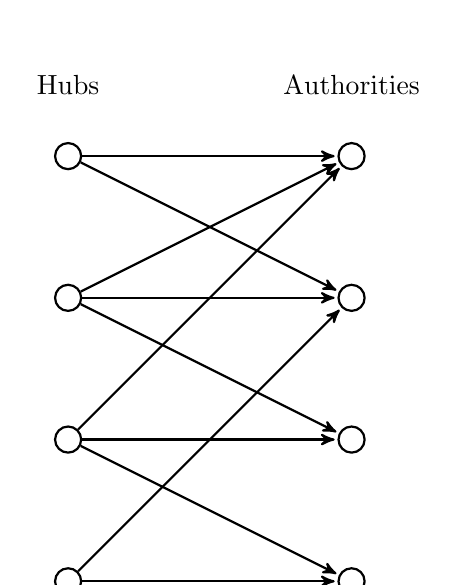
\begin{tikzpicture}[->,>=stealth',shorten >=1pt,auto,thick,scale=0.9]

% Hub nodes
\node[shape=circle,draw=black] (H1) at (0,6) {};
\node[shape=circle,draw=black] (H2) at (0,4) {};
\node[shape=circle,draw=black] (H3) at (0,2) {};
\node[shape=circle,draw=black] (H4) at (0,0) {};

% Authority nodes
\node[shape=circle,draw=black] (A1) at (4,6) {};
\node[shape=circle,draw=black] (A2) at (4,4) {};
\node[shape=circle,draw=black] (A3) at (4,2) {};
\node[shape=circle,draw=black] (A4) at (4,0) {};

% Arrows from hubs to authorities
\path (H1) edge (A1);
\path (H1) edge (A2);
\path (H2) edge (A1);
\path (H2) edge (A2);
\path (H2) edge (A3);
\path (H3) edge (A1);
\path (H3) edge (A3);
\path (H3) edge (A4);
\path (H4) edge (A2);
\path (H4) edge (A4);

% Labels
\node at (0,7) {Hubs};
\node at (4,7) {Authorities};

\end{tikzpicture}
\caption{Hubs and authorities hyperlink network, adapted from \cite{kleinberg_authoritative_1999}.}
\label{fig:hub-auth}
\end{figure}

We want the hub and authority scores to be mutually reinforcing: a page should have a high hub score if it links to many good authorities, and a high authority score if it is linked to by many good hubs.
To capture this, the weights are updated iteratively as follows:

\begin{equation*}
    a_p \gets \sum_{q:(q,p)\in E} h_q, \quad
    h_p \gets \sum_{q:(p,q)\in E} a_q \text{.}
\end{equation*}

\subsection{Psuedocode}
\begin{algorithm}[H]
\caption{HITS(G, k)}
\begin{algorithmic}[1]
\State $G$: a collection of $n$ linked pages $p$
\State $k$: a natural number of iterations
\State Initialize $a_p \gets 1$ and $h_p \gets 1$ for all $v \in G$
\For{$i = 1$ to $k$}
    \For{each $p \in G$}
        \State $a_p \gets \sum_{q:(q,p)\in E} h_q$
    \EndFor
    \For{each $p \in G$}
        \State $h_p \gets \sum_{q:(p,q)\in E} a_q$
    \EndFor
    \State Normalize $a$ and $h$ so $\sum_p a_p^2 = 1$ and $\sum_p h_p^2 = 1$
\EndFor
\State \Return ($a$, $h$)
\end{algorithmic}
\end{algorithm}

To ensure computational efficiency, we will pass our constructed $G_\sigma$ to HITS.
To return only the top $c$ authorities and hubs, we can modify the algorithm to report the pages with the $c$ largest values in $a$ and $h$ respectively.

\subsection{Proof of Convergence}
As one applies \texttt{HITS} to arbitrarily large values of $k$, the scores $a$ and $h$ converge to consistent (and, to the extent there is a correct answer, ``correct") sequences.

\begin{proof}
    Let $G = (V, E)$ with $V = \{p_1, p_2, \dots, p_n\}$, and let $A$ be the adjacency matrix of $G$.
    The update rules $a \gets A^T h$ and $h \gets A a$ imply that the sequence of hub vectors satisfies $h_k \propto (AA^T)^k z$ and the sequence of authority vectors satisfies $a_k \propto (A^T A)^{k-1} A^T z$ for initial vector $z$ of all 1s.

    Both $AA^T$ and $A^T A$ are real, symmetric, and positive semidefinite matrices.
    It follows from the power method (repeated updates of $h$ using $AA^T$ and normalization) that \textit{if $z$ has a nonzero component in the direction of the principal eigenvector of $AA^T$}, then $h_k$ converges to the unit vector in the direction of that eigenvector.
    Since $a_k$ is derived from $h_k$ via $a_k = A^T h_k$ and normalization, and $A^T$ is linear, $a_k$ also converges to the unit vector in the direction of the principal eigenvector of $A^TA$.
\end{proof}

In plain language, the authority and hub scores converge because they're being repeatedly multiplied by some transformation of the adjacency matrix.
With normalization to keep the numbers from blowing up, this procedure will eventually lead the scores to converge to the dominant eigenvector, reflecting the most prominent hubs and authorities.

\subsection{Runtime Analysis}
Let $n$ be the number of pages and $m$ be the number of links between them in the hyperlink graph. Let $k$ be the number of iterations.

Each authority score update runs in $O(m)$ time (summing over neighbors for all pages, equivalent to the number of links in the graph).
Likewise, each hub score updates runs in $O(m)$ time.
Therefore, each iteration runs in $O(2m) = O(m)$ time.

The total runtime is therefore $O(km)$, where $k$ is usually a small constant (\textcite{kleinberg_authoritative_1999} used 20) for convergence.

\section{Example}
\begin{figure}[ht]
    \centering

    \begin{minipage}{0.32\textwidth}
        \centering
        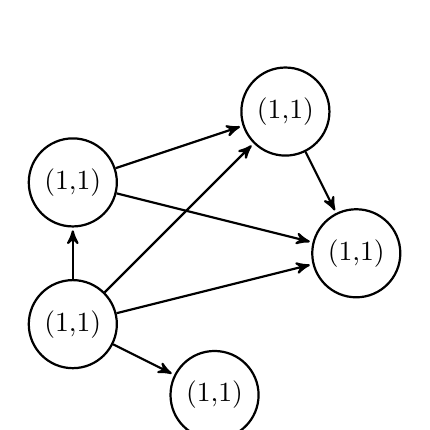
\begin{tikzpicture}[->,>=stealth',shorten >=1pt,auto,thick,scale=0.9]
        
            % Hub nodes
            \node[shape=circle,draw=black] (H1) at (0,5) {(1,1)};
            \node[shape=circle,draw=black] (H2) at (0,3) {(1,1)};
            
            % Authority nodes
            \node[shape=circle,draw=black] (A1) at (3,6) {(1,1)};
            \node[shape=circle,draw=black] (A2) at (4,4) {(1,1)};
            \node[shape=circle,draw=black] (A3) at (2,2) {(1,1)};
            
            % Arrows from hubs to authorities
            \path (H1) edge (A1);
            \path (H1) edge (A2);
            \path (H2) edge (A1);
            \path (H2) edge (A2);
            \path (H2) edge (A3);
            \path (A1) edge (A2);
            \path (H2) edge (H1);
        
        \end{tikzpicture}
        \caption*{\scriptsize Initial graph. Values are $(a, h)$.}
    \end{minipage}
    \hfill
    \begin{minipage}{0.32\textwidth}
        \centering
        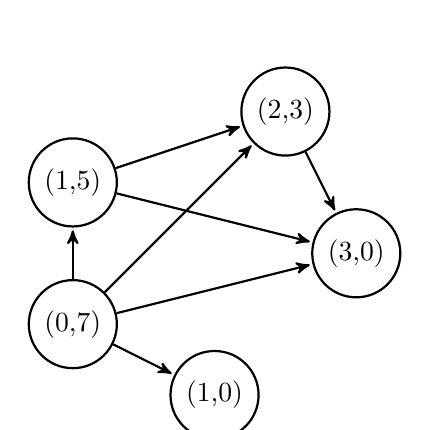
\begin{tikzpicture}[->,>=stealth',shorten >=1pt,auto,thick,scale=0.9]
        
            % Hub nodes
            \node[shape=circle,draw=black] (H1) at (0,5) {(1,5)};
            \node[shape=circle,draw=black] (H2) at (0,3) {(0,7)};
            
            % Authority nodes
            \node[shape=circle,draw=black] (A1) at (3,6) {(2,3)};
            \node[shape=circle,draw=black] (A2) at (4,4) {(3,0)};
            \node[shape=circle,draw=black] (A3) at (2,2) {(1,0)};
            
            % Arrows from hubs to authorities
            \path (H1) edge (A1);
            \path (H1) edge (A2);
            \path (H2) edge (A1);
            \path (H2) edge (A2);
            \path (H2) edge (A3);
            \path (A1) edge (A2);
            \path (H2) edge (H1);
        
        \end{tikzpicture}
        \caption*{\scriptsize One iteration, no normalization.}
    \end{minipage}
    \hfill
    \begin{minipage}{0.32\textwidth}
        \centering
        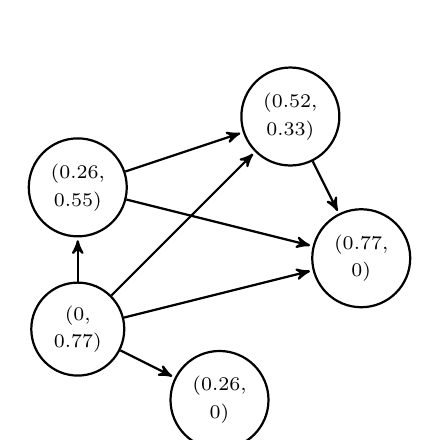
\begin{tikzpicture}[->,>=stealth',shorten >=1pt,auto,thick,scale=0.9]
        
            % Hub nodes
            \node[shape=circle,draw=black] (H1) at (0,5) {\scriptsize\shortstack{(0.26,\\0.55)}};
            \node[shape=circle,draw=black] (H2) at (0,3) {\scriptsize\shortstack{(0,\\0.77)}};
            
            % Authority nodes
            \node[shape=circle,draw=black] (A1) at (3,6) {\scriptsize\shortstack{(0.52,\\0.33)}};
            \node[shape=circle,draw=black] (A2) at (4,4) {\scriptsize\shortstack{(0.77,\\0)}};
            \node[shape=circle,draw=black] (A3) at (2,2) {\scriptsize\shortstack{(0.26,\\0)}};
            
            % Arrows from hubs to authorities
            \path (H1) edge (A1);
            \path (H1) edge (A2);
            \path (H2) edge (A1);
            \path (H2) edge (A2);
            \path (H2) edge (A3);
            \path (A1) edge (A2);
            \path (H2) edge (H1);
        
        \end{tikzpicture}
        \caption*{\scriptsize One iteration, with normalization.}
    \end{minipage}
    \caption{Initialization and one iteration of HITS.}
    \label{fig:hits-three}
\end{figure}

Figure \ref{fig:hits-three} shows the initial state of a toy model of a link graph, with one iteration and normalization step performed.
Doing this repeatedly would converge to the scores seen in Figure \ref{fig:hits-final}.
For this graph, with precision to two decimal places, four iterations is enough.
Given this data, we can conclude that the two nodes on the left are hubs, the three nodes on the right are authorities, and we can rank their quality relative to each other.

\begin{figure}
    \centering
    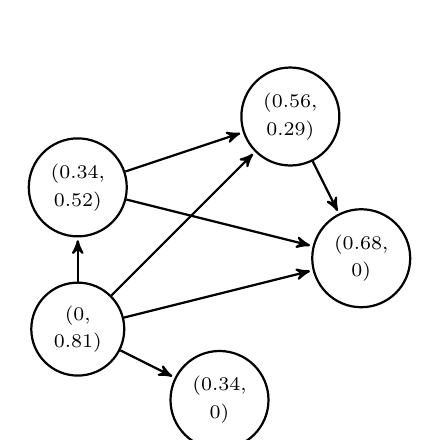
\begin{tikzpicture}[->,>=stealth',shorten >=1pt,auto,thick,scale=0.9]
    
        % Hub nodes
        \node[shape=circle,draw=black] (H1) at (0,5) {\scriptsize\shortstack{(0.34,\\0.52)}};
        \node[shape=circle,draw=black] (H2) at (0,3) {\scriptsize\shortstack{(0,\\0.81)}};
        
        % Authority nodes
        \node[shape=circle,draw=black] (A1) at (3,6) {\scriptsize\shortstack{(0.56,\\0.29)}};
        \node[shape=circle,draw=black] (A2) at (4,4) {\scriptsize\shortstack{(0.68,\\0)}};
        \node[shape=circle,draw=black] (A3) at (2,2) {\scriptsize\shortstack{(0.34,\\0)}};
        
        % Arrows from hubs to authorities
        \path (H1) edge (A1);
        \path (H1) edge (A2);
        \path (H2) edge (A1);
        \path (H2) edge (A2);
        \path (H2) edge (A3);
        \path (A1) edge (A2);
        \path (H2) edge (H1);
    
    \end{tikzpicture}
    \caption{Convergence of the toy example.}
    \label{fig:hits-final}
\end{figure}

\section{Conclusion}
The core insight of Hyperlink-Induced Topic Search -- that some websites are good at linking to other websites and some websites are good at providing content worth linking to -- allowed it to show worthwhile empirical results in searching the pre-Google internet.
However, HITS relies on selecting a good base set from a query, and is thus query-dependent and must be run at query time rather than indexing time.
Despite useful theoretical results, like fast convergence, it ultimately was not commonly used by search engines.
While HITS was immediately overshadowed by PageRank, it remains an interesting algorithm with an optimistic, somewhat antiquated, understanding of how information spreads online.

\section{References}
\printbibliography[heading=none]
Additionally, I used ChatGPT for brainstorming, outlining, content clarification, (extensive) \LaTeX\ assistance, and some coding and summarization tasks to efficiently move from my writeup to the presentation.
Those chatlogs can be audited here. Note that I was a little sloppy with keeping my other work separate, so there are a few non-relevant messages present. I apologize for the oversight!
\begin{itemize}
    \item \href{https://chatgpt.com/share/6819aca4-36d4-800f-b3ab-39e45524c3e7}{https://chatgpt.com/share/6819aca4-36d4-800f-b3ab-39e45524c3e7}
    \item \href{https://chatgpt.com/share/6819ae4f-63b4-800f-a159-33d2f44d3b50}{https://chatgpt.com/share/6819ae4f-63b4-800f-a159-33d2f44d3b50}
    \item \href{https://chatgpt.com/share/6819ae05-8bf8-800f-b9b5-df248e10e037}{https://chatgpt.com/share/6819ae05-8bf8-800f-b9b5-df248e10e037}
\end{itemize}

\end{document}
